\documentclass[a4paper,12pt,onesided]{report}
%Eigene Änderungen:
\usepackage{cite}
\usepackage[addtotoc]{abstract} %mit hinzufügen ins inhaltsverzeichnis
\usepackage[utf8]{inputenc}

%===========================================================
%== Definitionen fuer die Formatierung =====================
%===========================================================

% Use german names like "Literaturverzeichnis" instead of "Bibliography"
\usepackage{ngerman}

% Links inside of the document
%\usepackage{hyperref}

% Allows to use graphics
\usepackage{graphicx}

% Use times new roman and courier as fonts
\usepackage{times}
\usepackage{courier}

% Allow forcing positioning of floating figures
\usepackage{float}

% Allow special tye of configurable tables
\usepackage{tabularx}
\usepackage{multirow}


% Allows to change letter spcaing
\usepackage{microtype}

% Special table types
\usepackage{longtable}
\usepackage{colortbl}
\definecolor{gray}{gray}{0.85}


\usepackage[titles]{tocloft}


\usepackage{url}

\usepackage{listings}
\renewcommand*{\lstlistlistingname}{Codebeispielverzeichnis}
\renewcommand{\lstlistingname}{Code}
\lstset{frame=single,basicstyle=\footnotesize\bfseries\ttfamily,breaklines=true}

\usepackage{titlesec}
\titlespacing*{\chapter}{0pt}{-35pt}{0pt}

\lstset{numberbychapter=false}
\usepackage{chngcntr}
\counterwithout{figure}{chapter}
\counterwithout{table}{chapter}
\renewcommand{\tablename}{Tab.}

% Glossary
% More info here https://en.wikibooks.org/wiki/LaTeX/Glossary
\usepackage[toc]{glossaries}
\renewcommand*{\glossaryentrynumbers}[1]{}
\makeglossaries

% Some formatting stuff for "Praxisbericht"
\linespread{1.4}
\makeatletter
 \renewcommand*\l@section{\@dottedtocline{1}{0em}{2.3em}}
 \renewcommand*\l@subsection{\@dottedtocline{1}{1em}{2.3em}}
\makeatother
\usepackage[a4paper, left=2.5cm, right=2.5cm, top=2.5cm, bottom=2.5cm]{geometry}

\usepackage{fancyhdr}
\pagestyle{fancy}
\fancyfoot{}
\fancyfoot[R]{\thepage}
\fancyhead{}
\fancyhead[L]{\nouppercase{\leftmark}}
\fancypagestyle{plain}{\pagestyle{fancy}}



% for formatting titles of chapters
\usepackage{titlesec}

\titleformat{\chapter} % command
{\bfseries} % format
{\fontsize{16}{18}\selectfont \thechapter\ } % label
{0ex} % sep
{\fontsize{16}{18}\selectfont} % before-code
[] % after-code
\titleformat{\section} % command
{\bfseries} % format
{\fontsize{14}{16}\selectfont \thesection\ } % label
{0ex} % sep
{\fontsize{14}{16}\selectfont} % before-code
[] % after-code
\titleformat{\subsection} % command
{\bfseries} % format
{\fontsize{12}{14}\selectfont \thesubsection\ } % label
{0ex} % sep
{\fontsize{12}{14}\selectfont} % before-code
[] % after-code
 
% Linksbuendige Captions
\usepackage{caption}
\captionsetup{
  justification=raggedright,
  singlelinecheck=false
}

% Paragraph styles
\setlength{\parindent}{0cm}
\setlength{\parskip}{6pt}

% A todo macro for marking ToDos
\usepackage{color}
\newcommand{\todo}[1]{\textcolor{white}{\colorbox{red}{ To do %
       :}}\textcolor{red}{\ \ #1
   }\textcolor{red}{\colorbox{red}{III}}\ }




\begin{document}

% Titelseite
\begin{titlepage}
	\centering
	
\includegraphics[width=14.9cm]{img/logo}\\

	\fontsize{18}{20}\selectfont
	Hochschule für angewandte Wissenschaften Coburg\\[.1cm]
	Fakultät Elektrotechnik und Informatik\\[1.2cm]
	Studiengang: Informatik\\
	Bachelorarbeit\\[1.2cm]
	\fontsize{21}{23}\selectfont
	\textbf{Entwicklung einer hardwarebeschleunigten Berechnung der 
	Mandelbrotmenge auf einem FPGA}\\[1cm]
	\fontsize{18}{20}\selectfont
	von\\[1.2cm]
	Daniel Kirchner\\
	Matrikelnummer: 02219415\\[1.2cm]
	Abgabe der Arbeit: 15.07.2019\\[1.2cm]

	Betreut durch: Prof. Oliver Engel, Hochschule Coburg
\end{titlepage}

\begin{abstract}
	Im Rahmen dieser Bachelorarbeit wurde eine hardwarebeschleunigte Visualisierung der Mandelbrotmenge auf einem FPGA realisiert.
	Hierfür werden diverse mathematische und designtechnische Performanceoptimierungen vorgestellt, welche dann in einparalleles FPGA-Design implementiert wurden. Weiterhin sollen einige Eigenschaften und Besonderheiten der Mandelbrotmenge und von Fraktalen im Allgemeinen aufgezeigt werden.\\
	Das Projekt wurde für das Zybo Zynq-7000 Trainer Board entwickelt, welches über einen VGA-Output die Repräsentation des Fraktals in Form eines 800x600@60Hz Videosignals ausgibt. Zur optimalen Ausnutzung der auf diesem Board gegebenen Ressourcen (DSPs, BRAM) wurde die \textit{Vivado Design Suite} mit dem integrierten IP-Katalog verwendet.\\
\end{abstract}

% Inhaltsverzeichnis
{
  \setlength{\cftbeforechapskip}{-.5ex}
  \tableofcontents
  \addcontentsline{toc}{chapter}{Inhaltsverzeichnis}
}

% Abbildungsverzeichnis
\newpage
\listoffigures
\addcontentsline{toc}{chapter}{Abbildungsverzeichnis}

% Codeverzeichnis
\newpage
\lstlistoflistings
\addcontentsline{toc}{chapter}{Codebeispielverzeichnis}

% Abkuerzungsverzeichnis
\newpage
\section*{Abkürzungsverzeichnis}
\addcontentsline{toc}{chapter}{Abkürzungsverzeichnis}
\begin{tabular}{ll}
  JAX-RS&Java API for RESTful Web Services\\
  % TODO: updaten
\end{tabular}

% Beginn Arbeit
\newpage
\chapter{Einleitung}

%TODO vllt aufbau erklären
\section{Motivation}
Die stets wachsende Zahl von Komponenten die auf einem mikroelektronischen Bauteil pro Zeiteinheit untergebracht wird, ist ein Phänomen, welcbes Gordon Moore schon im Jahr 1965 aufgefallen ist \cite{moore1965cramming}. Die populäre, nach ihm benannte Beobachtung, dass die Anzahl der Transistoren pro integriertem Schaltkreis exponentiell mit der Zeit ansteigt ist allgemein als das Mooresche Gesetz bekannt.

Diese Gesetzlichkeit machte es möglich den stets wachsenden Leistungsanforderungen an moderne Hardware gerecht zu werden, indem immer mehr (und komplexere) identische Allzweck-Prozessoren (Kerne) pro CPU verbaut wurden.

Dieses Vorgehen kann jedoch nicht unbegrenzt lange betrieben werden, da die heute verwendeten MOS-Transistoren sich rapide ihren physikalischen Grenzen annähern. Ein besserer Umgang mit dem stetig steigenden Bedarf an Rechenleistung ist die Entwicklung von spezialisierter Hardware, welche zwar nur ein kleines Aufgabenspektrum abdeckt, dies jedoch mit hoher Performanz und Energieeffizienz tut.

Ein Beispiel hierfür ist die moderne Grafikkarte (GPU), welche dem Prozessor Darstellungsberchnungen abnimmt, wodurch dieser mehr Zeit hat, andere Aufgaben zu übernehmen. Die Grafikkarte führt diese Aufgaben mit enorm hohem Durchsatz und niedrigen Berechnungszeiten durch, welche ein herkömmlicher Prozessor alleine nicht erreichen könnte.

Auch andere Hardwarekomponenten, wie die Netzwerkkarte, kryptographische Beschleuniger, oder Soundkarten sind in fast allen Computersystemen verbaut und entlasten den Hauptprozessor. Man spricht auch von heterogenen Computersystemen.

Die im Rahmen dieser Arbeit vorgestellte Hardware soll ein Beispiel für eine derartige heterogene Komponente sein. Auf einem Field Programmable Gate Array (FPGA,) %TODO Kapitel linken
soll eine performante und energieffiziente Visualisierung der sogenannten Mandelbrotmenge realisiert werden. Diese Problemstellung ist auch durch einen ordinären Prozessor lösbar, lastet diesen jedoch enorm aus und ist somit auch sehr energieineffizient. %TODO Kapitel linken

\section{Aufgabenstellung}
Die Aufgabe dieses Projektes ist es, eine komplett in Hardware stattfindende Berechnung der Mandelbrotmenge durchzuführen und die Ergebnisse über eine VGA-Schnittstelle darzustellen (ähnlich Bild) %TODO
%TODO Mandelbrotmenge Bild

Weiterhin soll die Hardware durch externe Peripherie konfigurierbar hinsichtlich der angestellten Berechnungen sein. So soll etwa aktuell abgebildete Bereich der Mandelbrotmenge oder auch die Farbgebung der Darstellung im laufenden Betrieb geändert werden können.

Hierfür wurde das FPGA-Trainer Board \textit{Zybo Zynq-7000} zur Verfügung gestellt, welches in %TODO Kapitel linken
genauer vorgestellt wird.

\chapter{Technische Grundlagen}
Zum besseren Verständnis des Gesamtprojektes sollen in diesem Kapitel einige technische Konzepte erläutert werden.


\section{FPGAs}
Ein \textit{Field Programmable Gate Array} (kurz FPGA) ist ein Schaltkreis, welcher mit Hilfe von Hardwarebeschreibungssprachen %TODO Kapitel
konfiguriert werden kann, um beliebig komplexe logische Schaltungen zu realisieren.\\
Das Grundelement eines solchen Bausteines bilden die sogenannten \textit{Lookup Tables} (kurz LUTs), welche zu einem beliebigen n-bit Input ein 1-bit Output Signal produzieren. Die zugrundeliegende Logiktabelle einer LUT ist hierbei frei programmierbar.

\begin{figure}[H]
	\centering
	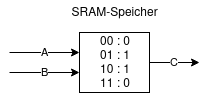
\includegraphics{LUT.png}
	\caption{Beispielhafter Aufbau einer 2-Input LUT}
	\label{fig:LUT}
\end{figure}

Eine LUT, welche die Operation $C = A \oplus B$ implementiert ist in \autoref{fig:LUT} zu sehen. In dieser wird in einem SRAM-Speicher für jede Inputkombination ein Outputwert hinterlegt, wodurch jede 2-Bit Funktion abgebildet werden kann. In Verbindung mit einem Flipflop \footnote{Ein Flipflop ist ein Speicherelement, welches einen einzigen Bit Daten halten kann.} bildet eine LUT dann einen sogenannten Logikblock (s. \autoref{fig:logikblock}).\cite{fpgaDesign}

\begin{figure}[H]
	\centering
	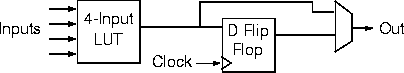
\includegraphics{logic_block.png}
	\caption{Logikblock, aus \cite{fpgaDesign}}
	\label{fig:logikblock}
\end{figure}

Ein FPGA verbindet nun durch ebenfalls konfigurierbare Bussysteme viele solcher Logikblöcke um komplexere Schaltkreise abzubilden.\\
Weiterhin verfügen FPGA-Boards oft noch über ergänzende Hardwarekomponenten, von denen die im Falle dieses Projektes vorhandenen im Folgenden gezeigt werden sollen.

\paragraph{DSP}
Ein \textit{Digitaler Signalprozessor} (DSP) ist ein fest integrierter Baustein, welcher durch Multiplizierer und Akkumulatoren binäre Algorithmen beschleunigt.
So übernimmt dieser etwa grundlegende mathematische Operationen, was dazu führt, dass diese flächen- und energiesparender durchgeführt werden, als bei der Verwendung von LUTs \cite[S. 52]{dsps}.
Typische Anwendungsgebiete dieser Bausteine sind Fließkommamultiplikationen, Schnelle Fourier-Transformationen oder einfache Zähler \cite[S. 14]{dsps}. 
In diesem Projekt wurden die DSPs hauptsächlich aufgrund ihrer 25x18 Bit Multiplizierer verwendet, welche kaskadiert werden können um beliebig Breite Multiplikationen durchzuführen.

\paragraph{Block RAM}
FPGAs verfügen meist über \textit{Block RAM} (BRAM), welcher zur Speicherung binärer Daten dient. Dieser Speicher ist lese-/schreibsynchron, wodurch Inkonsistenzen beim Speicherprozess ausgeschlossen sind \cite[S. 11]{dsps}. Um auf diese Speicherblöcke Zugriff zu erlangen muss der von Xilinx mitgelieferte Baustein "Block RAM Generator" verwendet werden.

\paragraph{IO-Komponenten}
Zur Kommunikation mit der Außenwelt verfügen FPGAs über diverse Schnittstellen wie z.B. Knöpfe, Schalter, aber auch komplexere Anbindungen wie etwa VGA (s. hierzu \autoref{chap:vga}) oder PMOD-Anschlüsse. %TODO Kapitel VGA verlinken
Diese sind so angebunden, dass ihre Signale direkt in Logikschaltungen von LUTs integriert werden können.

%TODO weitere wichtige komponenten


\section{VGA-Interface}
\label{chap:vga}

\chapter{Theoretische Grundlagen}
\section{Fraktale}
\section{Die Mandelbrotmenge}

\chapter{Test und Umsetzung}
	\section{Gesamtsystem}
	\section{Komponentenbeschreibung}
		\subsection{Mandelbrot-Core}
		\subsection{Mandelbrot-Koordinator}
		\subsection{Dual Port Block RAM}
		\subsection{Lookup Tables}
	\section{Peripherie und funktionale Beschreibung}

\chapter{Optimierungen}
	\section{Algebraische Optimierung}
	\section{Designoptimierungen}

% Literaturverzeichnis
\bibliography{bib}{}
\bibliographystyle{plain}

\end{document}